\subsection{Unlocking Forward Gain: Discover the Right S Parameter!}

\begin{tcolorbox}[colback=gray!10, colframe=black, title=E4B03`]
Which S parameter is equivalent to forward gain? 

\begin{enumerate}[label=\Alph*.]
    \item S11
    \item S12
    \item \textbf{S21}
    \item S22
\end{enumerate} \end{tcolorbox}

\subsubsection*{Concepts Related to the Question}

The question pertains to the parameters used in the analysis of linear electrical networks, specifically in the context of radio frequency (RF) communications. The S-parameters, or scattering parameters, are a set of measurements that describe the electrical behavior of linear electrical networks when undergoing various signal inputs and outputs. Each S-parameter denotes a specific relationship between incident and reflected power waves at the ports of a network.

1. \textbf{Forward Gain (S21)}: This parameter is used to measure the forward gain of a two-port network. S21 indicates how much of the input signal (applied at port 1) is transmitted to the output (observed at port 2). The value of S21 denotes the amplification and phase shift of the signal as it passes through the device.

2. \textbf{Reflected Power (S11/S22)}: These parameters denote how much of the incident power is reflected back to the source. S11 applies to port 1 (input), and S22 applies to port 2 (output). While these parameters are important in understanding losses and matching, they are not directly related to gain.

3. \textbf{Reverse Gain (S12)}: This parameter can be thought of as the reverse transmission gain from port 2 to port 1. It represents how much of the signal at port 2 can appear at port 1 when a signal is applied at port 2. This is less common in conventional forwarding scenarios.

Thus, among the options provided, 

\subsubsection*{Calculation Example}

Since the question specifically focuses on understanding S-parameters rather than requiring a numerical calculation, we can discuss the conceptual calculation of S21 as it involves:
- Measuring the incident power at port 1 (P1)
- Measuring the transmitted power observed at port 2 (P2)
  
The S-parameter can be calculated as:

\[
S_{21} = \frac{P_{2}}{P_{1}}
\]

Where:
- \(P_2\) is the power transmitted to port 2,
- \(P_1\) is the power incident at port 1.

\subsubsection*{Diagram Representation}

To illustrate this concept, we could draw a simple two-port network diagram using TikZ:

\begin{center}
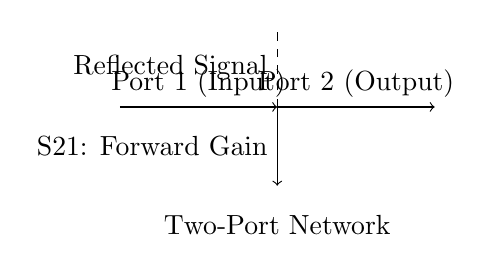
\begin{tikzpicture}
    \draw[->] (-2,0) -- (0,0) node[midway,above] {Port 1 (Input)};
    \draw[->] (0,0) -- (2,0) node[midway,above] {Port 2 (Output)};
    \draw[->] (0,0) -- (0,-1) node[midway,left] {S21: Forward Gain};
    \draw[dashed] (0,0) -- (0,1) node[midway,left] {Reflected Signal};
    \node at (0,-1.5) {Two-Port Network};
\end{tikzpicture}
\end{center}
